\documentclass{../../oss-handout}
\usepackage{newtxtext,newtxmath}
\usepackage{enumitem}
\usepackage{tikz}
\tikzset{>=latex}
\usetikzlibrary{patterns}

\setlength{\parindent}{0pt}
\setlength{\parskip}{6pt}
\setlength{\headheight}{26pt}

% Set the page style for the document
\pagestyle{plain}

% Course & Document information
\renewcommand{\institution}{Meritus Academy}
\renewcommand{\coursetitle}{Grade 12 Physics}
\renewcommand{\term}{Updated: Summer 2021}
\title{Class 5 Handout: Two-Object Elastic Collisions in One Dimension}
\author{Dr.\ Timothy Leung}

\date{\today}

\begin{document}
% Make the first page header and footer
\thispagestyle{title}

% Start the document
\gentitle

An \textbf{elastic collision} is a special case in which both \emph{momentum}
and \emph{kinetic energy} are conserved during the interaction. For simplicity,
this handout only deals with \emph{one-dimension} elastic collisions between
\emph{two} objects, as shown in Fig.~\ref{fig:1d}.
\begin{figure}[ht]
  \centering
  \begin{tikzpicture}[scale=.8]
    \tikzstyle{balloon1}=[ball color=red];
    \tikzstyle{balloon2}=[ball color=blue];
    \shade[balloon1](0,0) circle(1) node[white]{$m_1$};
    \draw[very thick,->](1,0)--(2.5,0) node[midway,above]{$v_1$};
    \shade[balloon2](7,0) circle(.6) node[white]{$m_2$};
    \draw[very thick,->](6.4,0)--(5.2,0) node[midway,above]{$v_2$};
  \end{tikzpicture}
  \caption{Collision of two objects in one dimension.}
  \label{fig:1d}
\end{figure}

\textbf{Conservation of momentum} is the direct consequence of the third law of
motion. During the collision, the two objects exert an equal and opposite force
on each other. Therefore, over the time interval $\Delta t$ of the collision,
an equal and opposite impulse ($J=F\Delta t$) is applied to each object. The
resulting change of momentum of each obiect is therefore equal and opposite,
and the net change of momentum is zero. In this case, the equation for
conservation of momentum equation can be expressed as:
\begin{equation}
  m_1v_{1i}+m_2v_{2i}=m_1v_{1f}+m_2v_{2f}
  \label{eq:mom1}
\end{equation}
where $m_1$ and $m_2$ are the masses of objects 1 and 2, $v_{1i}$ and $v_{2i}$
are, respectively, the initial velocities of the masses, and $v_{1f}$ and
$v_{2f}$ are their final velocities.

\textbf{Conservation of kinetic energy} results from the fact that during the
collision, conserative forces are present to transform kinetic energy into 
potential energy. This potential energy can be \emph{elastic}  (e.g.\ a spring 
that compresses when the two objects collide), \emph{electric} (e.g.\ two
charged particles moving towards each other), \emph{gravitational} (e.g.\
gravitational sling shots for satellites and deep-space vehicles), or
\emph{magnetic} (e.g.\ north poles of two magnets are repelled from each
other). In many cases, the objects never touch each other during the collision.
The conservative forces will then transform all the potential energy back into
kinetic energy. The result is that the total kinetic energies of both objects
before the collision is the same as the total afterwards, as shown
below\footnote{One of the most common comments by students
  is that Eq.~\ref{eq:K1} is the \emph{same} as Eq.~\ref{eq:mom1}. Clearly this
  is not the case! The momentum equation is \emph{linear} in $v$, while the
  kinetic energy equation is \emph{quadratic} in $v$.}:
\begin{equation}
  \frac12 m_1v_{1i}^2+\frac12m_2v_{2i}^2=\frac12 m_1v_{1f}^2+\frac12 m_2v_{2f}^2
  \label{eq:K1}
\end{equation}

To derive the equation for one-dimension elastic collisions, we collect
all the $m_1$ and $m_2$ terms in Eq.~\ref{eq:mom1} together. We can then move
all terms to the left hand side so that the right-hand side will be $1$, as
shown below:
\begin{align}
  m_1(v_{1i}-v_{1f})&=m_2(v_{2f}-v_{2i}) \label{eq:mom2a}\\
  \frac{m_1(v_{1i}-v_{1f})}{m_2(v_{2f}-v_{2i})}&=1 \label{eq:mom2}
\end{align}
Likewise, in the kinetic energy equation (Eq.\ \ref{eq:K1}), we can cancel all
the $\dfrac12$ factors from every term. Using the same approach
as the momentum equation, we collect the $m_1$ and $m_2$ terms together, and
then we factor the differences of squares terms\footnote{Remember the
  difference of squares: $(a^2-b^2)=(a+b)(a-b)$ in case you have forgotten. I
  sympathsize with you if you have indeed forgotten: there are so many things
  to remember from so many different courses!} on both sides of the equation.
Then the  terms are rearranged:
\begin{align}
  \nonumber m_1(v_{1i}^2-v_{1f}^2) &= m_2(v_{2f}^2-v_{2i}^2)\\
  \nonumber m_1(v_{1i}-v_{1f})(v_{1i}+v_{1f}) &= m_2(v_{2f}+v_{2i})(v_{2f}-v_{2i})\\
  \tikz[baseline]{
    \node[fill=blue!20] (n1) {
      $\left[\dfrac{m_1(v_{1i}-v_{1f})}{m_2(v_{2f}-v_{2i})}\right]$
    }
  }(v_{1i}+v_{1f}) &= (v_{2f}+v_{2i})
  \label{eq:K2}
\end{align}
Note that the highlighted term in Eq.~\ref{eq:K2} is just the left-hand-side
of Eq.~\ref{eq:mom2}, which is equal to $1$. We can therefore cancel all mass
terms and express the final velocities $v_{1f}$ and $v_{2f}$ in terms of other
velocities:
\begin{align}
  \nonumber  v_{1i}+v_{1f} &= v_{2f}+v_{2i}\\
  v_{2f}&=v_{1i}+v_{1f}-v_{2i}\quad\text{(solving for $v_{2f}$)}\label{eq:relvel1}\\
  v_{1f}&=v_{2i}+v_{2f}-v_{1i}\quad\text{(solving for $v_{1f}$)}\label{eq:relvel}
\end{align}
To solve for the final velocity of object 1, Eq.~\ref{eq:relvel1} is then
substituted back into Eq.~\ref{eq:mom2a}. This time, we collect all $v_{1i}$,
$v_{2i}$ and $v_{1f}$ terms together:
\begin{align}
  m_1(v_{1i}-v_{1f})&=m_2(v_{1i}+v_{1f}-v_{2i}-v_{2i})\\
  m_1v_{1i}-m_1v_{1f}&=m_2v_{1i}+m_2v_{1f}-2m_2v_{2i}\\
  (m_1-m_2)v_{1i}+2m_2v_{2i}&=(m_2+m_1)v_{1f}
  \label{eq:mom3}
\end{align}
By dividing every term in Eq.~\ref{eq:mom3} by the total mass ($m_2+m_1$), we 
obtain the final expression for the final velocity of object $1$:
\begin{equation}
  \boxed{
    v_{1f}=
    \left(\frac{m_1-m_2}{m_1+m_2}\right)v_{1i} +
    \left(\frac{2m_1}{m_1+m_2}\right)    v_{2i}
  }
  \label{eq:mom4}
\end{equation}
Likewise, Eq.~\ref{eq:relvel} can be substituted back into Eq.~\ref{eq:mom2a}
to obtain the expression for the final velocity of object 2:
\begin{equation}
  \boxed{
    v_{2f}=
    \left(\frac{2m_1}{m_1+m_2}\right)    v_{1i} +
    \left(\frac{m_1-m_2}{m_1+m_2}\right) v_{2i}
  }
  \label{eq:mom5}
\end{equation}
One special case is if the second object 2 is initially stationary, i.e.\
$v_{2i}=0$. In such a case, the $v_{2i}$ terms are dropped from
Eqs.~\ref{eq:mom4} and \ref{eq:mom5}, reducing the equations to:
\begin{align}
  v_{1f}&=\left(\frac{m_1-m_2}{m_1+m_2}\right)v_{1i}\\
  v_{2f}&=\left(\frac{2m_1}{m_1+m_2}\right)v_{1i}
  \label{eg:simple1}
\end{align}
There are a few different possibilities for outcomes:
\begin{itemize}[leftmargin=15pt]
\item\textbf{Two equal masses:} If the masses are equal, i.e.\ $m_1=m_2=m$,
  then Eq.~\ref{eg:simple1} becomes:
  \begin{align*}
    v_{1f}&=\left(\frac{m_1-m_2}{m_1+m_2}\right)v
    =\left(\frac{m-m}{m+m}\right)v=0\\
    v_{2f}&=\left(\frac{2m_1}{m_1+m_2}\right)v
    =\left(\frac{2m}{m+m}\right)v=v
  \end{align*}
  All the momentum and energy from object 1 is transferred to object 2. Object
  1 stops, while object 2 continues to move at $v$, as shown in
  Fig.~\ref{fig:same-mass}. This behaviour is most notably expressed in a
  \emph{Newton's cradle}.\footnote{Note that the Newton's cradle is \emph{not}
    an elastic collision. The fact that you can \emph{hear} the metal balls
    colliding means that energy has escaped the system as a sound wave.}
  \begin{figure}[ht]
    \centering
    \begin{tikzpicture}[scale=.8]
      \tikzstyle{balloon1}=[ball color=red];
      \tikzstyle{balloon2}=[ball color=blue];
      \shade[balloon1] (-1,0) circle(1) node[white]{$m$};
      \draw[very thick,->] (0,0)--(1.5,0) node[midway,above]{$v$};
      \shade[balloon2] (4,0) circle(1) node[white]{$m$};
      
      \shade[balloon1] (2,-2.5) circle(1) node[white]{$m$};
      \draw[dashed] (4,-2.5) circle(1);
      \draw[dashed] (5,-2.5)--(6,-2.5);
      \shade[balloon2] (7,-2.5) circle(1) node[white]{$m$};
      \draw[very thick,->] (8,-2.5)--(9.5,-2.5) node[midway,above]{$v$};
    \end{tikzpicture}
    \caption{When a moving object collides with a stationary object of equal
      mass, all the momentum and energy are transferred.}
    \label{fig:same-mass}
  \end{figure}
\item\textbf{Large Object Colliding With Small Object:} In this second case,
  object 1 is much more massive than the second object, i.e.\ $m_1\gg m_2$. We
  can then effectively ``ignore'' the $m_2$ terms in Eq.~\ref{eg:simple1}. The
  equations then become:
  \begin{align*}
    v_{1f}&=\left(\frac{m_1-m_2}{m_1+m_2}\right)v=\left(\frac{m_1}{m_1}\right)v
    =v\\
    v_{2f}&=\left(\frac{2m_1}{m_1+m_2}\right)v=\left(\frac{2m_1}{m_1}\right)v=2v
  \end{align*}
  Object 1 continues to move at nearly its initial speed $v$, while object 2
  picks up \emph{twice} the speed of object 1, as shown in
  Fig~\ref{fig:big-small}. This kind of collision is often used in
  gravitational slingshots, which forms the basis for deep-space exploration
  probes that need to travel through the solar system.
  \begin{figure}[ht]
    \centering
    \begin{tikzpicture}[scale=.8]
      \tikzstyle{balloon1}=[ball color=red];
      \tikzstyle{balloon2}=[ball color=blue];
      \shade[balloon1](0,0) circle(1.5) node[white]{$m_1$};
      \draw[very thick,->](1.5,0)--(3,0) node[midway,above]{$v$};
      \shade[balloon2](7,0) circle(.6) node[white]{$m_2$};
      
      \shade[balloon1](5.5,-2.5) circle(1.5) node[white]{$m_1$};
      \draw[very thick,->](7,-2.5)--(8.5,-2.5) node[midway,above]{$v$};
      \draw[dashed](7,-2.5) circle(.6);
      \draw[dashed](7.6,-2.5)--(9.4,-2.5);
      \shade[balloon2](10,-2.5) circle(.6) node[white]{$m_2$};
      \draw[very thick,->](10.6,-2.5)--(13.6,-2.5) node[midway,above]{$2v$};
    \end{tikzpicture}
    \caption{When a large object collides with a stationary small object, 
    it does not slow down, but the smaller object gains twice the speed.}
    \label{fig:big-small}
  \end{figure}
\item\textbf{Small Object Colliding With Large Object:} In this final case,
  object 1 has a much smaller mass than object 2, i.e.\ $m_1\ll m_2$. Like the
  previous case, we can effectively ignore the smaller mass, which is $m_1$ in
  this case. Then, Eq.~\ref{eg:simple1} reduces to:
  \begin{align*}
    v_{1f}&=\left(\frac{m_1-m_2}{m_1+m_2}\right)v=\left(\frac{-m_2}{m_2}\right)v
    =-v\\
    v_{2f}&=\left(\frac{2m_1}{m_1+m_2}\right)v=\left(\frac{2m_1}{m_2}\right)v=0
  \end{align*}
  Object 2 continues to be stationary, while object 1 bounces back at its
  original speed, as shown in Fig~\ref{fig:big-small}.
  \begin{figure}[ht]
    \centering
    \begin{tikzpicture}[scale=.8]
      \tikzstyle{balloon1}=[ball color=red];
      \tikzstyle{balloon2}=[ball color=blue];
      \shade[balloon1](0,0) circle(.5) node[white]{$m_1$};
      \draw[very thick,->](.5,0)--(2,0) node[right]{$v$};
      \shade[balloon2](7,0) circle(1.5) node[white]{$m_2$};
    
      \shade[balloon1](4,-3.3) circle(.5) node[white]{$m_1$};
      \draw[very thick,->](3.5,-3.3)--(2,-3.3) node[left]{$v$};
      \shade[balloon2](7,-3.3) circle(1.5) node[white]{$m_2$};
    \end{tikzpicture}
    \caption{When a small objects collides with a stationary large object, it
      bounces back with the same speed, while the larger object remains
      stationary.}
  \end{figure}
\end{itemize}
\end{document}

